\chapter{Signals}

The signal system is implemented to somewhat comfort with \acs{POSIX} threads
and process signaling. This means that signals can be sent to both processes as
well as threads. Signals are passed to signal receiving entities in forwarding
fashion, a bit like how packet forwarding could work.

\section{Userspace signal handlers}

Figure \ref{figure:sigstack} shows how entry to a user space signal handler
constructs necessary data on top of the user stack and alters the thread
stack frame.

\begin{figure}
  \center
  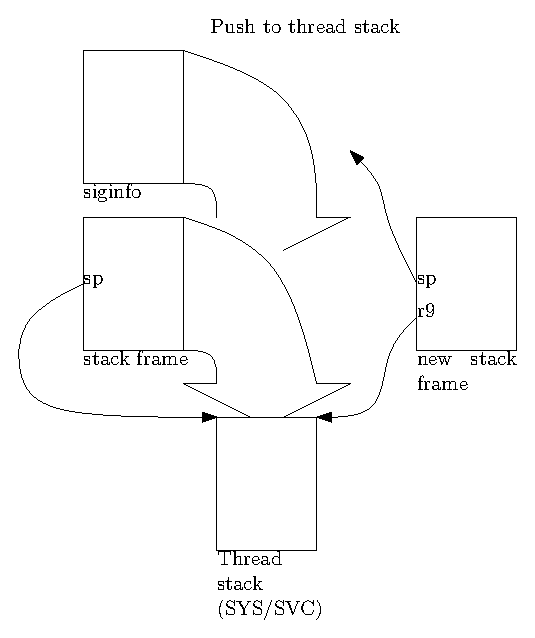
\includegraphics[width=7cm]{pics/signal_stack}
  \caption{A signal stack and the new thread stack frame.}
  \label{figure:sigstack}
\end{figure}

Figure \ref{figure:syscallint} shows the signal handling flow when
a signal is received in a middle of a system call and the system call
is interrupted to immediately run the user space signal hanlder.

\begin{figure}
\begin{verbatim}
  \/        usr | kernel
+-----------+           +---------+
| syscall() |------...->| sys_xxx | <- KSIGFLAG_SIGHANDLER
+-----------+           +---------+    syscall handler interrupted
                |              |
                               \/
+-------------+ |   +------------------------+
| sig_handler |<----| ksignal_syscall_exit() |  
+-------------+ |   +------------------------+
       |
       \/       |
+-------------+     +---------------------+
| sigreturn() |---->| sys_signal_return() |
+-------------+ |   +---------------------+
                              |
                |            /
 return to <-----------------
 the original   |
 syscall() on top (EINTR)
\end{verbatim}
\caption{Interruption of a system call when a signal is caught.}
\label{figure:syscallint}
\end{figure}
